\documentclass[11pt,preprint, authoryear]{elsarticle}

\usepackage{lmodern}
%%%% My spacing
\usepackage{setspace}
\setstretch{1.2}
\DeclareMathSizes{12}{14}{10}{10}

% Wrap around which gives all figures included the [H] command, or places it "here". This can be tedious to code in Rmarkdown.
\usepackage{float}
\let\origfigure\figure
\let\endorigfigure\endfigure
\renewenvironment{figure}[1][2] {
    \expandafter\origfigure\expandafter[H]
} {
    \endorigfigure
}

\let\origtable\table
\let\endorigtable\endtable
\renewenvironment{table}[1][2] {
    \expandafter\origtable\expandafter[H]
} {
    \endorigtable
}


\usepackage{ifxetex,ifluatex}
\usepackage{fixltx2e} % provides \textsubscript
\ifnum 0\ifxetex 1\fi\ifluatex 1\fi=0 % if pdftex
  \usepackage[T1]{fontenc}
  \usepackage[utf8]{inputenc}
\else % if luatex or xelatex
  \ifxetex
    \usepackage{mathspec}
    \usepackage{xltxtra,xunicode}
  \else
    \usepackage{fontspec}
  \fi
  \defaultfontfeatures{Mapping=tex-text,Scale=MatchLowercase}
  \newcommand{\euro}{€}
\fi

\usepackage{amssymb, amsmath, amsthm, amsfonts}

\usepackage[round]{natbib}
\bibliographystyle{natbib}
\def\bibsection{\section*{References}} %%% Make "References" appear before bibliography
\usepackage{longtable}
\usepackage[margin=2.3cm,bottom=2cm,top=2.5cm, includefoot]{geometry}
\usepackage{fancyhdr}
\usepackage[bottom, hang, flushmargin]{footmisc}
\usepackage{graphicx}
\numberwithin{equation}{section}
\numberwithin{figure}{section}
\numberwithin{table}{section}
\setlength{\parindent}{0cm}
\setlength{\parskip}{1.3ex plus 0.5ex minus 0.3ex}
\usepackage{textcomp}
\renewcommand{\headrulewidth}{0.2pt}
\renewcommand{\footrulewidth}{0.3pt}

\usepackage{array}
\newcolumntype{x}[1]{>{\centering\arraybackslash\hspace{0pt}}p{#1}}

%%%%  Remove the "preprint submitted to" part. Don't worry about this either, it just looks better without it:
\makeatletter
\def\ps@pprintTitle{%
  \let\@oddhead\@empty
  \let\@evenhead\@empty
  \let\@oddfoot\@empty
  \let\@evenfoot\@oddfoot
}
\makeatother

 \def\tightlist{} % This allows for subbullets!

\usepackage{hyperref}
\hypersetup{breaklinks=true,
            bookmarks=true,
            colorlinks=true,
            citecolor=blue,
            urlcolor=blue,
            linkcolor=blue,
            pdfborder={0 0 0}}


% The following packages allow huxtable to work:
\usepackage{siunitx}
\usepackage{multirow}
\usepackage{hhline}
\usepackage{calc}
\usepackage{tabularx}
\usepackage{booktabs}
\usepackage{caption}
\usepackage{colortbl}

\urlstyle{same}  % don't use monospace font for urls
\setlength{\parindent}{0pt}
\setlength{\parskip}{6pt plus 2pt minus 1pt}
\setlength{\emergencystretch}{3em}  % prevent overfull lines
\setcounter{secnumdepth}{5}

%%% Use protect on footnotes to avoid problems with footnotes in titles
\let\rmarkdownfootnote\footnote%
\def\footnote{\protect\rmarkdownfootnote}
\IfFileExists{upquote.sty}{\usepackage{upquote}}{}

%%% Include extra packages specified by user
% Insert custom packages here as follows
% \usepackage{tikz}

%%% Hard setting column skips for reports - this ensures greater consistency and control over the length settings in the document.
%% page layout
%% paragraphs
\setlength{\baselineskip}{12pt plus 0pt minus 0pt}
\setlength{\parskip}{12pt plus 0pt minus 0pt}
\setlength{\parindent}{0pt plus 0pt minus 0pt}
%% floats
\setlength{\floatsep}{12pt plus 0 pt minus 0pt}
\setlength{\textfloatsep}{20pt plus 0pt minus 0pt}
\setlength{\intextsep}{14pt plus 0pt minus 0pt}
\setlength{\dbltextfloatsep}{20pt plus 0pt minus 0pt}
\setlength{\dblfloatsep}{14pt plus 0pt minus 0pt}
%% maths
\setlength{\abovedisplayskip}{12pt plus 0pt minus 0pt}
\setlength{\belowdisplayskip}{12pt plus 0pt minus 0pt}
%% lists
\setlength{\topsep}{10pt plus 0pt minus 0pt}
\setlength{\partopsep}{3pt plus 0pt minus 0pt}
\setlength{\itemsep}{5pt plus 0pt minus 0pt}
\setlength{\labelsep}{8mm plus 0mm minus 0mm}
\setlength{\parsep}{\the\parskip}
\setlength{\listparindent}{\the\parindent}
%% verbatim
\setlength{\fboxsep}{5pt plus 0pt minus 0pt}



\begin{document}

\begin{frontmatter}  %

\title{Theory of Statistics Likelihood Assigment}

\author[Add1]{Sean Soutar STRSEA001}
\ead{sean.soutar@gmail.com}

\author[Add2]{Fabio Fehr FHRFAB001}
\ead{FHRFAB001@myuct.ac.za}




\address[Add1]{UCT Statistics Honours, Cape Town, South Africa}
\address[Add2]{UCT Statistics Honours, Cape Town, South Africa}


\begin{abstract}
\small{
This project will explore the Accidents dataset and try fit a Poisson,
Negative Binomial, Mixture of 2 Poissons and zero inflated Poisson
models to the data. The model with the strongest support will be chosen
and discussed. Profile likelihoods and confidence intervals for the
parameters will be found and displayed of the chosen model.
}
\end{abstract}

\vspace{1cm}

\begin{keyword}
\footnotesize{
Likelihood \sep Overdispersion \sep Soek \\ \vspace{0.3cm}
\textit{JEL classification} 
}
\end{keyword}
\vspace{0.5cm}
\end{frontmatter}



%________________________
% Header and Footers
%%%%%%%%%%%%%%%%%%%%%%%%%%%%%%%%%
\pagestyle{fancy}
\chead{}
\rhead{}
\lfoot{}
\rfoot{\footnotesize Page \thepage\\}
\lhead{}
%\rfoot{\footnotesize Page \thepage\ } % "e.g. Page 2"
\cfoot{}

%\setlength\headheight{30pt}
%%%%%%%%%%%%%%%%%%%%%%%%%%%%%%%%%
%________________________

\headsep 35pt % So that header does not go over title




\section{Introduction}\label{introduction}

This assignment is an explorative report on a dataset containing the
number of accidents on two-lane (same direction) road segments in Cape
Town over a five-year period. The segments differ in length between 0.2
and 7.2 km. The aim of the report is to find and fit a model which
accurately describes the accident dataset. This report will first
explore the data then fit different adequate distributions and choose
the most appropriate one. Once a model has been selected the profile
likelihood and confidence intervals will be programmed and calculated
from from first principles. The results will then be analysed critically
and conclusions will be made and consider further considerations in the
study.

\subsection{Exploratory data analysis}\label{exploratory-data-analysis}

To better understand our data this report shall explore the following
properties; Firstly we examine the type of data within the accidents
dataset and discuss whether our data is discrete ordinal or continuous.
After the symmetry of the data and bounds will be discussed. This leads
the exploration to outliers and extreme values.

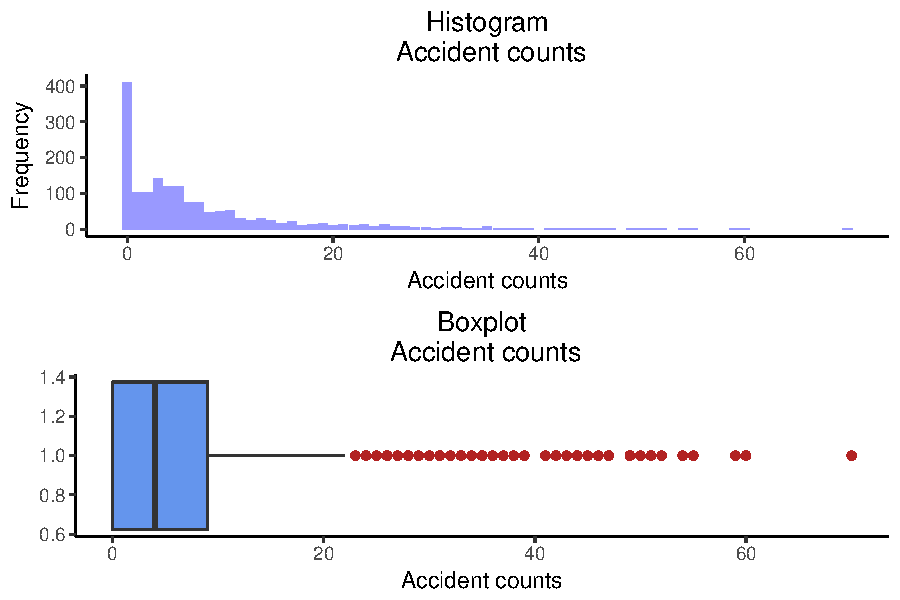
\includegraphics{likelihood_files/figure-latex/unnamed-chunk-1-1.pdf}

\subsubsection{\texorpdfstring{Data type
\label{data_description}}{Data type }}\label{data-type}

There are many instances where zero accidents were observed. This
accounts for approximately 25.18\% of the data. This suggests that the
zero-inflated Poisson should be considered as this proportion is much
higher than what would be expected of a regular Poisson distribution.
The accident counts are discrete random variables. Specifically, they
are discrete positive definite random variables on the interval
\(R \in \{0;+ \infty\}\). Summary statistics of the data are shown
below.

\begin{longtable}[]{@{}rrr@{}}
\caption{Summary statisitics}\tabularnewline
\toprule
Mean & Variance & Median\tabularnewline
\midrule
\endfirsthead
\toprule
Mean & Variance & Median\tabularnewline
\midrule
\endhead
6.9179 & 85.0858 & 4\tabularnewline
\bottomrule
\end{longtable}

In the Poisson distribution, the mean should equal the variance. The
sample variance far exceeds the sample mean. This indicates
overdispersion if the Poisson distribution were to be used. This is when
the observations are more variable than what would be expected. This
suggests that alternative count models and mixture distributions should
be used.

\subsubsection{Symmetry}\label{symmetry}

This property is visually seen in the histogram and boxplot. All counts
are greater than zero with a median value of 4 accidents. The largest
accident observed is 70 accidents. THe histogram shows that the data are
non-symetrical and positively skewed which is usually expected of count
data.

\subsubsection{Outliers}\label{outliers}

From the boxplot it clear that many outliers exist. One common method of
classifying a point as an extreme value or outlier is if it falls more
than 1.5 times the inner-quartile range above the upper quartile. The
proportion of outliers within our data set amount to 15.26\%.

\section{Methods}\label{methods}

\subsection{Model Formulation}\label{model-formulation}

The data is discrete, asymmetric, positive definite, contains many
positive outliers and many zeros. This would suggest distributions such
as Poisson, Negative Binomial, mixture distribution of 2 Poissons and a
zero inflated Poisson.

\subsection{Akiake Information Coefficient
(AIC)}\label{akiake-information-coefficient-aic}

The AIC metric can be used to compare models from different families of
distributions. They can be used to compare relative goodness of fit
between models. Overfitting the model with too many parameter is
penalised by an increased AIC, thus a lower AIC value indicates a better
fitting model.

\begin{align*}
\text{AIC} &= -2l(\hat{\theta}) + 2\text{p} \\
p &= \text{Number of estimated parameters}
\end{align*}

\subsection{Bayesian Information Criterion
(BIC)}\label{bayesian-information-criterion-bic}

This metric, like AIC, also compares relative goodness of fit between
models but penalises complex models when the sample size is large. BIC
tends to produce simpler models than AIC.

\begin{align*}
\text{BIC} &= -2l(\hat{\theta}) + log(n) \\
n &= \text{Number of observations}
\end{align*}

\subsection{Model Distributions}\label{model-distributions}

\subsubsection{Poisson}\label{poisson}

\begin{align*} 
p(x) & =  \frac{e^{-\lambda} \lambda^x}{x!},\ \ x\in \{0,1,\ldots,\infty\},\lambda>0 \\
\\
L(\lambda|x) & = \prod_{i=1}^n p(x_i) \\
\\
L(\lambda|x) & =\dfrac{e^{-n\lambda}\lambda^{\sum_{i=1}^n x_i}}{\prod_{i=1}^n x_i!}\\
\\
l(\lambda|x) & =-n\lambda +  \left(\sum_{i=1}^n x_i\right)\ln \lambda - \sum_{i=1}^{n}\ln(x_i!)
\end{align*}

The Poisson is characterised by the \(\lambda\) parameter which denotes
the population average rate of event occurence. In this context it would
be the average number of accidents per unit time frame.

\begin{longtable}[]{@{}rrr@{}}
\caption{Poisson MLE's \& information metrics}\tabularnewline
\toprule
\(\hat{\lambda}\) & AIC & BIC\tabularnewline
\midrule
\endfirsthead
\toprule
\(\hat{\lambda}\) & AIC & BIC\tabularnewline
\midrule
\endhead
6.9179 & 20263.64 & 20269.04\tabularnewline
\bottomrule
\end{longtable}

\subsubsection{Negative Binomial}\label{negative-binomial}

\begin{align*} 
p(x) & =  {\frac {\Gamma (r+x)}{x!\,\Gamma (r)}}\left({\frac {m}{r+m}}\right)^{x}\left({\frac {r}{r+m}}\right)^{r}\quad {\text{for }}x=0,1,2,\dotsc \\
\\
L(m,r|x) & = \prod_{i=1}^n p(x_i) \\
\\
L(m,r|x) & ={[\frac{1}{\Gamma (r)}]}^{n} \prod_{i=1}^{n}{\frac{\Gamma (r+x_i)}{x_{i}!}} (\frac{m}{r + m})^{\Sigma_{i=1}^n x_i} (\frac{r}{r + m})^{nr}   \\
\\
l(m,r|x) & = -n\ln[\Gamma (r)] + \sum^{n}_{i=1} \ln(\Gamma (r + x_i)) -\sum^{n}_{i=1}\ln x_i! + \sum^{n}_{i=1} x_{i} \ln (\frac{m}{r + m}) + nr \ln (\frac{r}{r + m})
\end{align*}

This parameterisation of the negative binomial is characterised by the
mean parameter m and the shape parameter r. It is important to note that
the variance of a Negative Binomial under this parameterisationg is
\(m + \frac{m^2}{r}\). Shape parameters are often regarded as nuisance
parameters and do not play a meaningful role in maximising likelihood.
Therefore, since we desire no under or over dispersion, we can express
the shape parameter as a function of the mean parameter to be esimated
and the sample variance.

CHECK THIS! LOOK AT PAPER CALLED ESTIMATING SHAPE. I HAVE HIGHLIGHTED
SOME STUFF ON SECOND PAGE

\begin{align*}
Var(x) &= m + \frac{m^2}{r} \\
r &= \frac{m^2}{Var(x) - m} \\
\hat{r} &= \frac{\hat{m}^2}{S^2 - \hat{m}}
\end{align*}

\begin{longtable}[]{@{}rrrr@{}}
\caption{Negative Binomial MLE's \& information metrics}\tabularnewline
\toprule
Mean \(\hat{m}\) & Shape \(\hat{r}\) & AIC & BIC\tabularnewline
\midrule
\endfirsthead
\toprule
Mean \(\hat{m}\) & Shape \(\hat{r}\) & AIC & BIC\tabularnewline
\midrule
\endhead
6.8108 & 0.5926 & 9626.917 & 9630.314\tabularnewline
\bottomrule
\end{longtable}

\subsubsection{Mixture of 2 Poissons}\label{mixture-of-2-poissons}

A finite mixture distributon of two Poisson variables will now be
explored. A possibly reason for the overdispersion is that the data are
from two separate Poisson distributions. Since it is not known from
which distribution that any given data point is from, presuming that the
two distribution mixture is appropriate, an additional mixing parameter
\(p\) needs to be estimated.

\begin{align*} 
p(x|\lambda_1,\lambda_2,p) & =  p\frac{e^{-\lambda_1} \lambda_1^x}{x!} + (1-p)\frac{e^{-\lambda_2} \lambda_2^x}{x!},\ \ x\in \{0,1,\ldots,\infty\},\lambda_1 , \lambda_2 , p >0 \\
\\
L(\lambda_1,\lambda_2,p|x) & = \prod_{i=1}^n p(x_i) \\
\\
L(\lambda_1,\lambda_2,p|x) & =  \prod_{i=1}^n p\frac{e^{-\lambda_1} \lambda_1^{x_i}}{x_i!} + (1-p)\frac{e^{-\lambda_2} \lambda_2^{x_i}}{x_i!} \\
\\
l(\lambda_1,\lambda_2,p|x) & \sum^n_{i=1} \ln [ p\frac{e^{-\lambda_1} \lambda_1^{x_i}}{x_i!} + (1-p)\frac{e^{-\lambda_2} \lambda_2^{x_i}}{x_i!} ]
\end{align*}

The parameters \(\lambda_1\) and \(\lambda_2\) refer to the average
number of road accidents per road stretch for the first and second
distribution respectively. The parameter p is the mixing parameter. This
represents the probability that a given observation belongs to
distribution 1. Therefore, the probability that an observation belongs
to distribution 2 is the \(1-p\) quantity.

\begin{longtable}[]{@{}rrrrr@{}}
\caption{Poisson-Poisson MLE's \& information metrics}\tabularnewline
\toprule
\(\hat{\lambda_1}\) & \(\hat{\lambda_2}\) & Proportion p & AIC &
BIC\tabularnewline
\midrule
\endfirsthead
\toprule
\(\hat{\lambda_1}\) & \(\hat{\lambda_2}\) & Proportion p & AIC &
BIC\tabularnewline
\midrule
\endhead
19.3809 & 2.8407 & 0.2465 & 12075.12 & 12076.52\tabularnewline
\bottomrule
\end{longtable}

\subsubsection{Zero inflated Poisson}\label{zero-inflated-poisson}

The Zero Inflated Poisson is also a finite mixture distribution. This
model supposes that the data can come from two distributions. The one is
a Zero Process and the other is a Poisson process that can only take on
non-zero values. This model is useful if there are many zeroes in the
data. This was seen to be the case as discussed in
\ref{data_description}. The Zero Inflated Poisson is a piecewise defined
distribution with different mass functions for predicting the
probability that a given observation will be zero rather than non-zero.

\begin{align*}
p(x_{i}=0) &= \pi +(1-\pi )e^{{-\lambda }} \\
\\
p(x_{i} \neq 0) &=(1-\pi ){\frac  {\lambda ^{{x_{i}}}e^{{-\lambda }}}{x_{i}!}},\qquad x_{i}\geq 1 \\
\\
L(\lambda,\pi|x) &= L(\lambda,\pi |x = 0)L(\lambda,\pi|x \neq 0)
\end{align*}

An indicator variable \(I\) is defined. \[ 
I =\begin{cases} 
      0 & x=0 \\
      1 & x \neq 0
   \end{cases}
\]

\begin{align*}
L(\lambda,\pi|x) &= \prod^{n}_{i=1} p(x_{i}=0)^{1 - I}p(x_{i} \neq 0)^{I} \\
\\
L(\lambda,\pi|x) &= \prod^{n}_{i=1} [\pi +(1-\pi )e^{{-\lambda }}]^{1 - I}[(1-\pi ){\frac  {\lambda ^{{x_{i}}}e^{{-\lambda }}}{x_{i}!}}]^{I} \\
\\
l(\lambda,\pi|x) &= \sum^{n}_{i=1} \ln[(1-I)[\pi +(1-\pi )e^{{-\lambda }}] + I[(1-\pi ){\frac  {\lambda ^{{x_{i}}}e^{{-\lambda }}}{x_{i}!}}]]
\end{align*}

The parameter \(\lambda\) is the average rate of accidents per road
stretch. The parameter \(\pi\) is the probability of extra zeroes in the
data. MAYBE EXPLAIN THIS BETTER?

\begin{longtable}[]{@{}rrrr@{}}
\caption{Zero inflated Poisson MLE's \& information
metrics}\tabularnewline
\toprule
\(\hat{\lambda}\) & \(\hat{\pi}\) & AIC & BIC\tabularnewline
\midrule
\endfirsthead
\toprule
\(\hat{\lambda}\) & \(\hat{\pi}\) & AIC & BIC\tabularnewline
\midrule
\endhead
9.2456 & 0.2518 & 15556.16 & 15559.56\tabularnewline
\bottomrule
\end{longtable}

\subsection{Model Selection}\label{model-selection}

The AIC and BIC results for each model are summarised below.

\begin{table}

\caption{\label{tab:aic_summary}Models fitted to accident data}
\centering
\begin{tabular}[t]{lrr}
\toprule
Model & AIC & BIC\\
\midrule
Poisson & 20263.641 & 20269.039\\
\textbf{Negative Binomial} & \textbf{9626.917} & \textbf{9630.314}\\
Poisson Mixture & 12075.122 & 12076.520\\
Zero Inflated Poisson & 15556.157 & 15559.555\\
\bottomrule
\end{tabular}
\end{table}

The Negative Binomial has the lowest AIC value at 9626.92. This implies
that is the best fitting model when compared to the other three models.
The goodness of the Negative Binomial fit will now be assessed further.

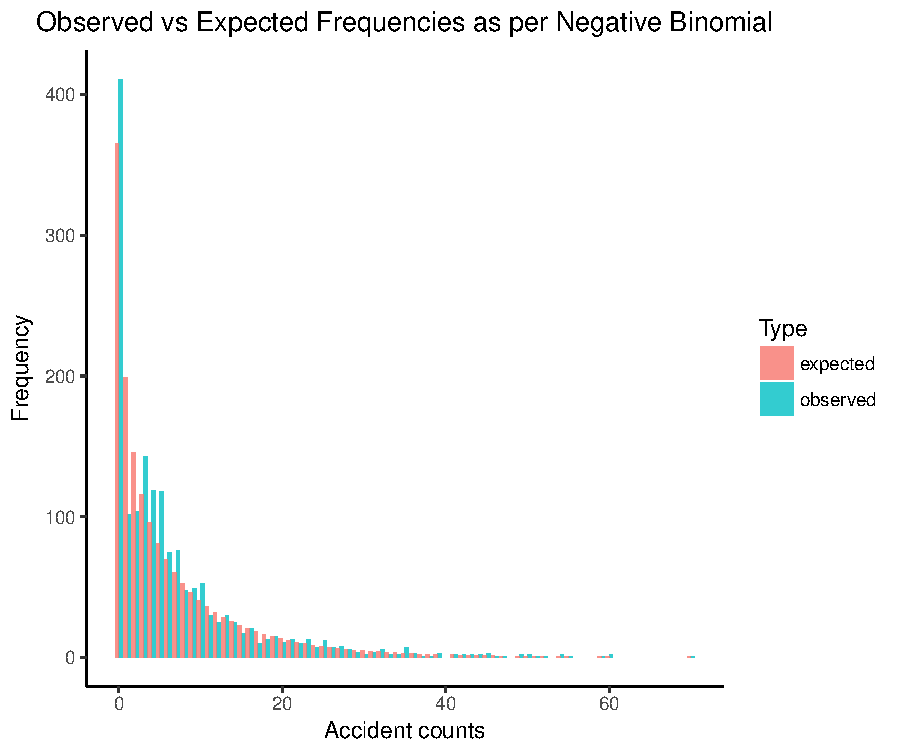
\includegraphics{likelihood_files/figure-latex/best_model_fit-1.pdf}

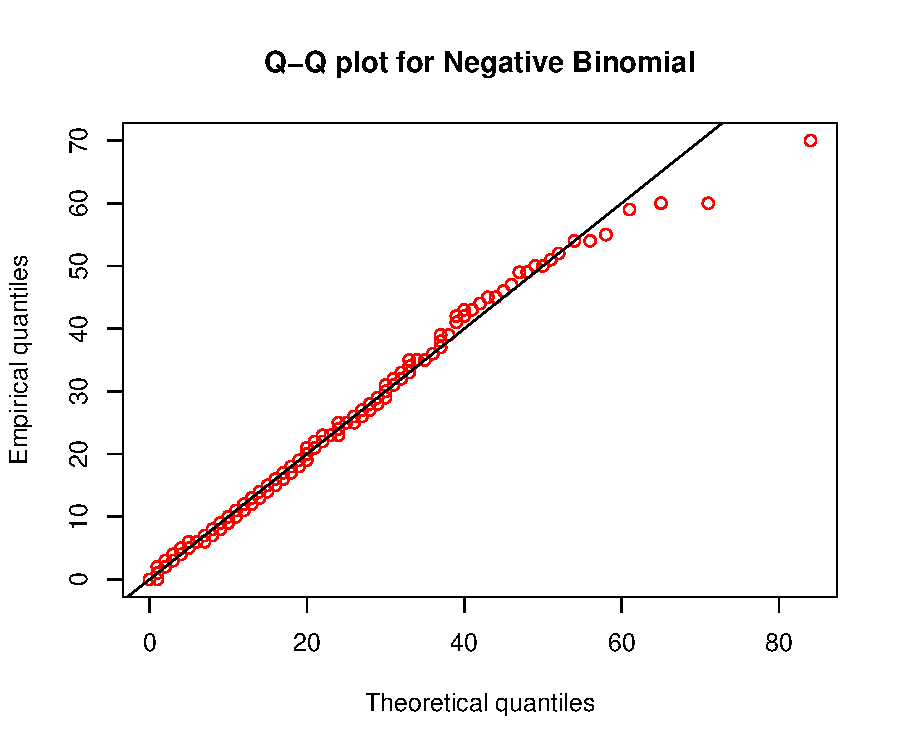
\includegraphics{likelihood_files/figure-latex/qq_plot-1.pdf}

\begin{verbatim}
## 
##  Pearson's Chi-squared test
## 
## data:  filter(comparison_df, Type == "observed")$Frequency and filter(comparison_df, Type != "observed")$Frequency
## X-squared = 1456, df = 1430, p-value = 0.3101
\end{verbatim}

\subsection{Profile Likelihood \& Confidence
Intervals}\label{profile-likelihood-confidence-intervals}

The profile likelihood is a techinque used to estimate the likelihood
function of a single parameter when multiple parameters are estimated
simultaenously. The profile likelihoods for the m and r parameters are
calculated as follows:

\begin{align*}
\end{align*}

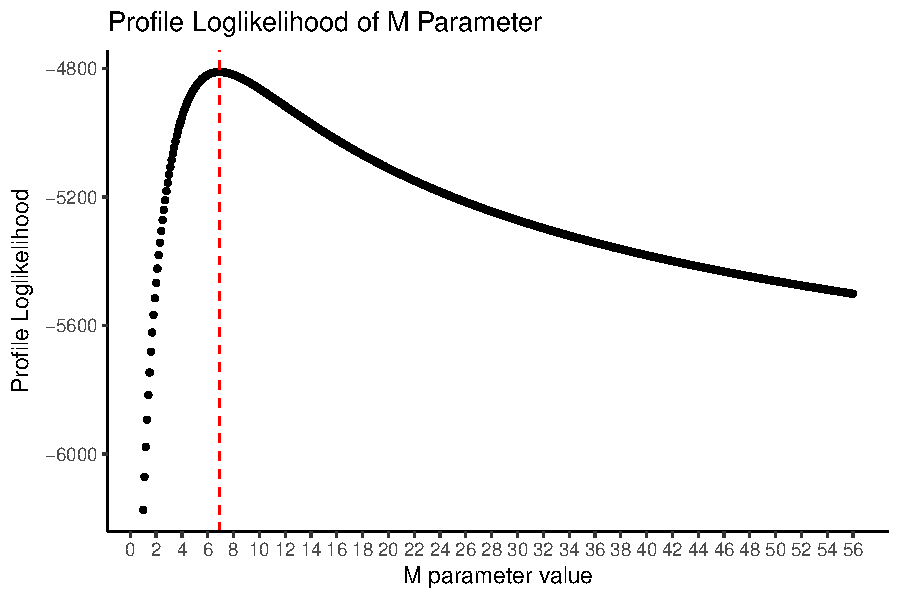
\includegraphics{likelihood_files/figure-latex/profile_likelihood_m-1.pdf}

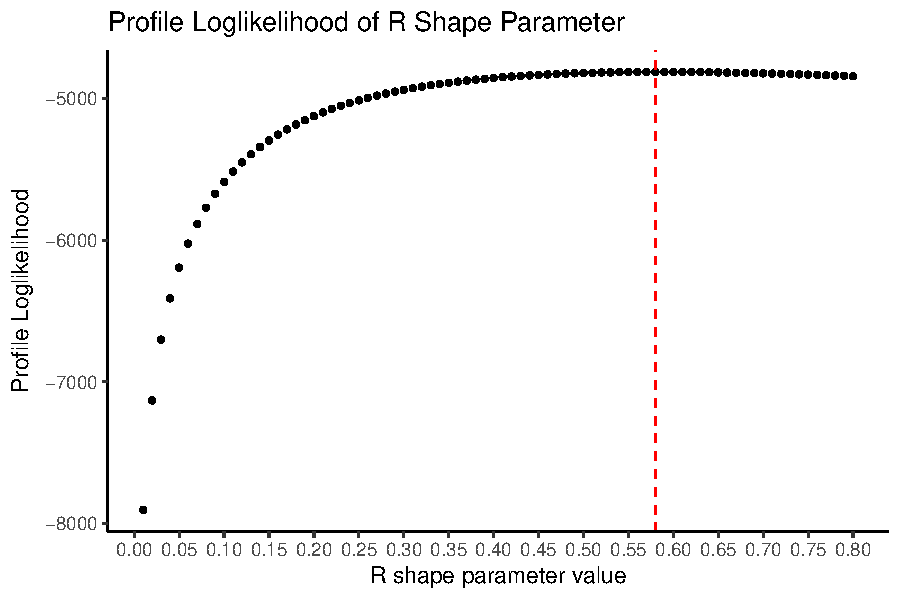
\includegraphics{likelihood_files/figure-latex/profile_likelihood_r-1.pdf}

It can be seen that the profile likelihood for the M parameter is
somewhat quadratic , but this is clearly not the case for the R shape
parameter. Therefore it would be inappropriate to use a Wilks Likelihood
interval or Wald interval for the shape parameter. The direct likelihood
interval should be used. However, the quadracity of the M parameter
profile likelihood means that asymptotic intervals relying on quadracity
could be used.

\section{Results}\label{results}

\textless{}\textless{}\textless{}\textless{}\textless{}\textless{}\textless{}
Updated upstream

======= -Are parameter estimates correlated?
\textgreater{}\textgreater{}\textgreater{}\textgreater{}\textgreater{}\textgreater{}\textgreater{}
Stashed changes

\section{Conclusion}\label{conclusion}

-What are the next steps and how can we improve the models

\section{References}\label{references}

% Force include bibliography in my chosen format:
\newpage
\nocite{*}
\bibliography{}





\end{document}
